\documentclass{sig-alternate-ipsn13}



\usepackage{color}
\usepackage{listings}
\usepackage{amsmath}


\newcommand{\nats}{\ensuremath{\mathbb{N}}}

\lstset{
  language=haskell,
  basicstyle=\footnotesize\ttfamily,breaklines=true,
  frame=none,
  literate=
    {->}{{$\rightarrow\;$}}1
    {=>}{{$\Rightarrow\;$}}1
    {++}{{\code{++}}}1
    {~}{{\ }}1
    {\\dollar}{{$\$$\;}}1,
  % Style for (listings') identifiers
  identifierstyle={\ttfamily\color{black}},
  % Style for declaration keywords
  keywordstyle=[1]{\ttfamily\color{violet}},
  % Style for gallina keywords
  keywordstyle=[2]{\ttfamily\color{green}},
  % Style for sorts keywords
  keywordstyle=[3]{\ttfamily\color{blue}},
  % Style for tactics keywords
  keywordstyle=[4]{\ttfamily\color{blue}},
  % Style for terminators keywords
  keywordstyle=[5]{\ttfamily\color{red}},
  morekeywords=[1]{class, instance},
  morekeywords=[2]{where},
  morekeywords=[3]{Maybe},
  morekeywords=[4]{main},
  morekeywords=[6]{do, proc, last, first, try, idtac, repeat},
}



\begin{document}

\title{A Sample {\ttlit ACM} SIG Proceedings Paper in LaTeX
Format\titlenote{(Does NOT produce the permission block, copyright information nor page numbering). Supported by ACM.}}
%
% You need the command \numberofauthors to handle the 'placement
% and alignment' of the authors beneath the title.
%
% For aesthetic reasons, we recommend 'three authors at a time'
% i.e. three 'name/affiliation blocks' be placed beneath the title.
%
% NOTE: You are NOT restricted in how many 'rows' of
% "name/affiliations" may appear. We just ask that you restrict
% the number of 'columns' to three.
%
% Because of the available 'opening page real-estate'
% we ask you to refrain from putting more than six authors
% (two rows with three columns) beneath the article title.
% More than six makes the first-page appear very cluttered indeed.
%
% Use the \alignauthor commands to handle the names
% and affiliations for an 'aesthetic maximum' of six authors.
% Add names, affiliations, addresses for
% the seventh etc. author(s) as the argument for the
% \additionalauthors command.
% These 'additional authors' will be output/set for you
% without further effort on your part as the last section in
% the body of your article BEFORE References or any Appendices.

\numberofauthors{4} %  in this sample file, there are a *total*
% of EIGHT authors. SIX appear on the 'first-page' (for formatting
% reasons) and the remaining two appear in the \additionalauthors section.
%
\author{
% You can go ahead and credit any number of authors here,
% e.g. one 'row of three' or two rows (consisting of one row of three
% and a second row of one, two or three).
%
% The command \alignauthor (no curly braces needed) should
% precede each author name, affiliation/snail-mail address and
% e-mail address. Additionally, tag each line of
% affiliation/address with \affaddr, and tag the
% e-mail address with \email.
%
% 1st. author
\alignauthor
Ben Trovato\titlenote{Dr.~Trovato insisted his name be first.}\\
       \affaddr{Institute for Clarity in Documentation}\\
       \affaddr{1932 Wallamaloo Lane}\\
       \affaddr{Wallamaloo, New Zealand}\\
       \email{trovato@corporation.com}
% 2nd. author
\alignauthor
G.K.M. Tobin\titlenote{The secretary disavows
any knowledge of this author's actions.}\\
       \affaddr{Institute for Clarity in Documentation}\\
       \affaddr{P.O. Box 1212}\\
       \affaddr{Dublin, Ohio 43017-6221}\\
       \email{webmaster@marysville-ohio.com}
\and  % use '\and' if you need 'another row' of author names
% 3rd. author
\alignauthor Lars Th{\o}rv{\"a}ld\titlenote{This author is the
one who did all the really hard work.}\\
       \affaddr{The Th{\o}rv{\"a}ld Group}\\
       \affaddr{1 Th{\o}rv{\"a}ld Circle}\\
       \affaddr{Hekla, Iceland}\\
       \email{larst@affiliation.org}
% 4th. author
\alignauthor Lawrence P. Leipuner\\
       \affaddr{Brookhaven Laboratories}\\
       \affaddr{Brookhaven National Lab}\\
       \affaddr{P.O. Box 5000}\\
       \email{lleipuner@researchlabs.org}
}

\maketitle
\begin{abstract}

Machine learning has been leveraged to great effect in the construction of efficient and performant cyber physical systems.
However, this has introduced the problem of legibility - it is hard to make formal arguments about the behavior of learned systems.
We propose an approach to structured machine learning by leveraging reactive program synthesis.

\end{abstract}

\section{Introduction}

Autonomous vehicles are considered to be one of the most challenging
types of reactive systems currently under development~\cite{AlurMT16,
  WongpiromsarnKF11, RamanDSMS15}. They need to interact reliably with
a highly reactive environment and crashes cannot be tolerated.  Life
critical decisions have to be made instantaneously and need to be
executed at the right point in time.

The development of autonomous vehicles and other cyberphysical systems
is supported by a wide spectrum of
programming and modelling methodologies, 
including synchronous programming languages like Lustre~\cite{conf/popl/CaspiPHP87} 
and Esterelle~\cite{conf/concur/BerryC84},
hardware-oriented versions of imperative programming languages like
SystemC~\cite{open2006ieee}, and visual languages like MSCs and Stateflow-charts~\cite{harel2003message,journals/scp/Harel87}.
The question of which programming paradigm is best-suited to write
easy-to-understand, bug-free code is still largely unresolved.

In the development of other forms of critical software, outside the
embedded domain, developers increasingly turn to functional
programming (cf.~\cite{frankau2009commercial}).  The strong type system in functional
languages largely eliminates runtime errors~\cite{cardelli1996type}.
Higher-order functions like \texttt{map} often eliminate the need for
explicit index counters, and, hence, the risk of ``index out of
bounds'' errors.  Functional purity reduces the possibility of
malformed state that can cause unexpected behavior.

While mathematical models of embedded and cyberphysical systems often
rely on functional notions such as stream-processing
functions~\cite{DBLP:series/mcs/BroyS01,DBLP:conf/csdm/Broy12}, the
application of functional programming in the practical development of
such systems has, so far, been limited. One of the most advanced
programming language in this direction is Ivory, which was used in the
development autonomous vehicles~\cite{pike2014}.  Ivory is a
restricted version of the C programming language, embedded in Haskell.
It provides access to the low level operations necessary for embedded
system programming, but still enforces good programming practice, such
as disallowing pointer arithmetic, with a rich type system.

Ivory does not, however, have an explicit notion of time.
It cannot then deal directly with the integration of 
continuous and discrete time, which is fundamental for the
development of a cyberphysical system. For example,
in a car, continuous signals, such as the velocity or acceleration,
mix with the discrete steps of the digital controller.

In this paper, we investigate the use of functional programming
in a domain where the interaction between continuous and discrete signals
is of fundamental importance. We build a vehicle controller capable
of both autonomous vehicle control and multi-vehicle communication,
such as the coordination in platooning situations.

Our approach is based on Functional Reactive Programming
(FRP)~\cite{hudak2003arrows,hudak2000haskell}.
The fundamental idea of FRP is to extend the classic building blocks 
of functional programming (\eg monads, arrows,
applicatives)
with the abstraction of a \emph{signal} to
describe time-varying values. FRP programs can be exceptionally
efficient.  For example, a network controller recently implemented as
an FRP program on a multicore processor outperforms any other such
controller existing today~\cite{Voellmy:2012:SSD:2377677.2377735}.

We have built a library, \ourLib, to use FRP to control a vehicle inside a simulation.
The library interfaces Haskell FRP programs to TORCS, The Open Racing Car Simulator, an open-source vehicle simulator~\cite{torcs}.
TORCS has been used in the Simulated Car Racing Championship competition~\cite{SCRC}, as well as other autonomous vehicle research projects~\cite{xu2016experimental,OnievaPAMP09,conf/cig/CardamoneLL09,conf/cig/MunozGS10}. 
Through \ourLib, the Haskell program has access to the sensors and actuators of the car, as well
as the communication channels between different vehicles.
Such a simulator is a  critical component of modern autonomous vehicle research, especially towards the goal of safe platooning algorithms~\cite{kamali2016formal}.

We report on experience with a case study, in which we implement a controller for a car on an empty race trace. 
Our controller successfully navigates the TORCS preloaded tracks with a reasonable speed and finesse, similar to that expected of an average driver (see Fig.~\ref{fig:race}). 
Furthermore, the case study illustrates that the functional approach indeed leads to elegant, easily understandable, and safe code.

\begin{figure}[t]
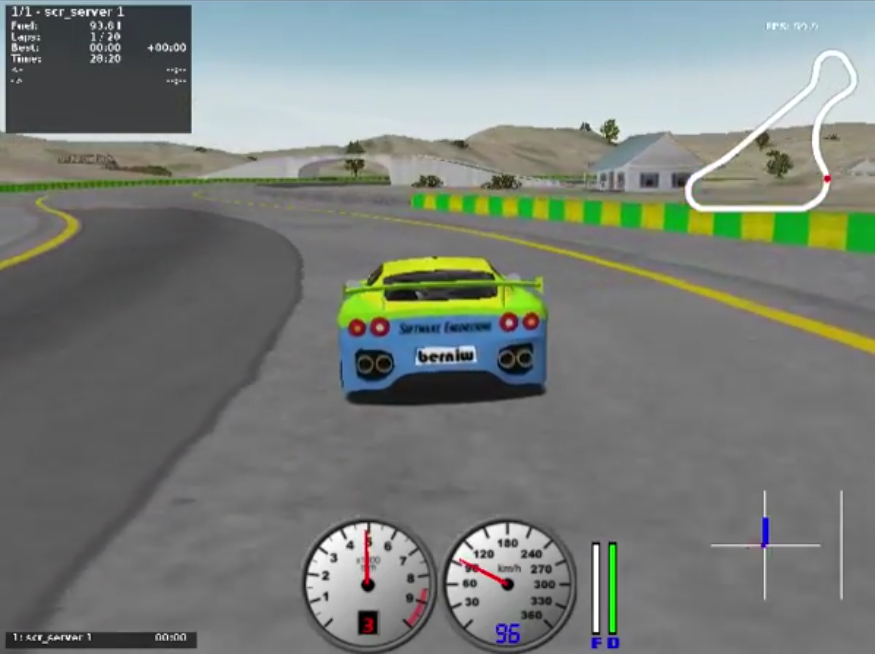
\includegraphics[width=0.45\textwidth]{figs/racing.png}
\caption{A screenshot of Haskell controlling the autonomous vehicle in the TORCS simulator}
\label{fig:race}
\end{figure}


\section{Motivating Example}

We take as a motivating example, the gearing controller component for an autonomous vehicle system.
In a typical scenario, we might build a neural network to control the output of the gear box at every time step based on all relevant sensor data.
We then have a neural network, $\fullNN$, processing inputs (acceleration, braking, speed, rpm, gear) to produce a new (gear) signal.

We can imagine this as a mealy machine with a single state and a single transition, which is always active.

\begin{figure}[h!]
\centering
\begin{tikzpicture}[shorten >=1pt,node distance=2.8cm,on grid]
  \node[state]   (q_0)                {$q_0$};
  \path[->] (q_0) 
		  edge [loop above]   node  [above,align=center]         {$\top,$\\$ \fullNN$} ();
\end{tikzpicture}
\caption{A mealy machine of a single monolithic neural network}
\label{fig:full}
\end{figure}

Now assume we have some adversarial actor that takes control of the speed sensor.
Since this network is processing the speed signal at every time step, we cannot have any guarantee of the effect a faulty speed sensor will have on our overall output.

In contrast, imagine we build an automata of neural networks as below.
Here, we have composed three networks; $\isAccel$ for a binary classifier that indicates whether the car is accelerating and the two multiclass classifiers, $\rpmGear$ and $\speedGear$, mapping their inputs to the target gear into which the car should shift (for example gears 1-5).
The mealy machine says that when the car is not accelerating, we should not shift the gear.
It also specifies that when we start to accelerate after a period of slowing down, we should set the gear based on the current speed.
As the car continues to accelerate, the gear should be set based on the rpm of the engine.

\begin{figure}[h!]
\centering
\begin{tikzpicture}[shorten >=1pt,node distance=2.8cm,on grid]
  \node[state]   (q_0)                {$q_0$};
  \node[state] (q_1) [right=of q_0] {$q_1$};
  \path[->] (q_0) 
		  edge [loop left]   node  [above,align=center]         {$\neg \isAccel,$\\$ \varnothing$} ()
		  edge [bend left=45] node [above,align=center] {$\isAccel,$\\$ \rpmGear$} (q_1)
            (q_1) 
		  edge [loop right]   node [above right,xshift=-0.5cm,align=center]        {$\isAccel,$\\$ \speedGear$} ()
		  edge [bend left=45] node [below,align=center] {$\neg \isAccel,$\\$ \varnothing$} (q_0);
\end{tikzpicture}
\caption{A mealy machine of multiple composed neural networks}
\label{fig:components}
\end{figure}

In Fig.~\ref{fig:components}, we clearly see that an attack on the speed sensor is guaranteed to only have an effect on the transition from state $q_0$ to state $q_1$.
Because of this compartmentalization of vulnerability, safety tactics such as trying to detect anomalous values may be employed to greater effect.
In the sequel, we will present a quantitative formalization of the vulnerability of the systems in both Fig.~\ref{fig:full} and Fig.~\ref{fig:components}.


\section{Saftey}

In this section, building off the definition provided in~\cite{DBLP:journals/corr/HuangKWW16}, we provide a formal definition of the vulnerability to advererial input of a mealy machine where the transition actions are neural networks.
We then show how by decomposing a larger neural network into an automata of smaller neural networks, we can reduce the overall vulnerability of the system.
Relying on the structure of the automata connecting the network, we can provide formal proofs activation periods of each individual network and demonstrate that adversarial inputs are less likely to be acted upon within a given time frame.


\section{Parameterized Synthesis}

We show how FRP synthesis can be parameterized over pure function implementations, thereby providing a nice target for combination with machine learning.


\section{Case Study: TORCS}

We use the Haskell bindings to TORCS to synthesize an FRP controller for a autonomous vehicle.
Since our synthesis procedure requires implementations of the pure functions to be complete, we leave those details to machine learning.

\subsection{Specifying a Driver}

\subsection{Optimization}
As a simpler case, we first provide rough implementations of the pure functions, leaving out only the critical values such as target speed and turning radius.
We use stochastic gradient descent to find optmimal values (where the cost is the lap time) to be embedded in the pure functions.


\subsection{Full Synthesis}
In this section we demonstrate how to use a nueral network to generate the low level interpretation of the pure functions to machine learning.
In this way, we still rely on the formalized program synthesis to give us a correct by construction framework for the driver.




\section{Related Work}

TORCS has been used as a simulator for formal verification of platoons~\cite{kamali2016formal}, etc... \cmark{TODO pick a few TORCS paper from google scholar}.
None of these works have used FRP as the language for the controller.


FRP specifically has been proposed as a tool for vehicle control~\cite{kazemi2016,zou2016}.
This work extends FRP to also prioritize certain functions for timing constraints.
This has been not yet been tested on vehicle simulation, in part due to the lack of a simulator compatible with the FRP language model.

FRP has been used for embedded systems~\cite{helbling2016juniper} and networking~\cite{voellmy2012scalable}.
The FRP networking library took advantage of Haskell's multicore support and significantly outperformed competing tools written in C++ and Java.


To the best of our knowledge this is the first FRP-based vehicle simulator.
Although there are many bindings to various vehicle simulators, these tend to use imperative languages.
For instance, TORCS allows users to directly edit the source code and add a new car in C++.
There are also TORCS bindings for python, java, and matlab, which have been used in the SCRC competition~\cite{SCRC}.

The videogame GTA~\cite{} has also been used to train image recognition software for autonomous vehicles~\cite{}.
While GTA is professionally produced game, which has more attractive graphics and a more advanced physics engine, it has a different set of issues.
First, is that as proprietary software that was not designed for autonomous vehcile reserach, the ability to build sensor based controllers is more restricted. 
Furthermore, unlike TORCS, which is designed primarily as a vehicle simulator, GTA's physics engine is tuned to maximize entertainment.
Using GTA as a meaningful control simulator would still be valuable work, but we leave this to future explorations.


\section{Conclusions}

\subsection{Future Work}

Since DFA are equivalent to Recurrent Neural Networks in expressibility, it would be interesting to replace the Mealy machine as a gating network with a RNN.
It is possible that,in practice, the particular structure of the gating network is more powerful than required. 
Instead, just by defining the subnetworks (the experts), this may be sufficient to maintain some safety properties.

In our analysis we have only viewed this problem from a verification perspective. 
An additional complexity is the actual learning rate and effectiveness of such a network structure.
We know that the Mixture of Experts architecture can be used to reduce the training time in general, but so far we have not explored the effect of using a Mealy machine as the gating network on the learning process.
Such an analysis is more well-suited to the machine learning community.


%ACKNOWLEDGMENTS are optional
\section*{Acknowledgments}
Acknowledgement goes here.

%
% The following two commands are all you need in the
% initial runs of your .tex file to
% produce the bibliography for the citations in your paper.
\bibliographystyle{abbrv}
\bibliography{sigproc}  % sigproc.bib is the name of the Bibliography in this case
% You must have a proper ".bib" file
%  and remember to run:
% latex bibtex latex latex
% to resolve all references
%
% ACM needs 'a single self-contained file'!
%
%APPENDICES are optional
%\balancecolumns
\appendix
%Appendix A

Appendix goes here.

% That's all folks!
\end{document}
